\section{SMT Model}
This section describes our SMT approach for the Sports Tournament Scheduling (STS) problem.  
The problem is modeled using the Quantifier-Free Linear Integer Arithmetic (QF\_LIA) theory and solved with the SMT solvers Z3 and CVC5.  
Our encoding is divided into two phases.

In \textbf{Phase~1}, we generate a feasible round-robin schedule by selecting a valid assignment of precomputed matches to each slot. The matches for each week are determined in advance using the matrix $rb$. Each slot $(p,w)$ then chooses one of these predefined pairs.

In \textbf{Phase~2}, we optimize the feasible solution by balancing the number of home and away games for each team.  
Each phase is encoded in a separate \texttt{.smt2} instance.

\subsection{Decision Variables}

\textbf{Phase~1:}
\begin{itemize}
    \item $\mathit{home}_{p,w} \in \{1,\dots,n\}$: home team assigned to period $p$ in week $w$.
    \item $\mathit{away}_{p,w} \in \{1,\dots,n\}$: away team assigned to period $p$ in week $w$.
    \item $\mathit{index}_{p,w,t} \in \{\text{true}, \text{false}\}$: true if pair $t$ is selected for slot $(p,w)$.
\end{itemize}

\textbf{Phase~2:}
\begin{itemize}
    \item $\mathit{flip}_{p,w} \in \{\text{true}, \text{false}\}$: true if the home and away teams in slot $(p,w)$ are swapped to improve balance.
    \item $\mathit{homeEff}_{p,w}$, $\mathit{awayEff}_{p,w}$: effective home and away teams after possible flipping.
\end{itemize}

\subsection{Objective Function}

The objective function applies only to \textbf{Phase~2} and aims to minimize the maximum imbalance $k$ between home and away games for any team:
\[
k^* = \min \Big\{\, k ~\Big|~ \forall\, t,\; |H_t - A_t| \leq k\, \Big\},
\quad H_t = \sum_{p,w} [\,\mathit{homeEff}_{p,w} = t\,], \quad
A_t = \sum_{p,w} [\,\mathit{awayEff}_{p,w} = t\,].
\]

The effective assignments are defined by:
\[
\mathit{homeEff}_{p,w} = \text{ite}(\mathit{flip}_{p,w},\, \mathit{away}_{p,w},\, \mathit{home}_{p,w}), \quad
\mathit{awayEff}_{p,w} = \text{ite}(\mathit{flip}_{p,w},\, \mathit{home}_{p,w},\, \mathit{away}_{p,w}).
\]

The optimal $k^*$ is found via binary search over the feasible imbalance bounds.

\subsection{Constraints}

\textbf{Phase~1:}
\begin{itemize}
    \item \textbf{Unique pair selection:} each slot $(p,w)$ must select exactly one pair $t$:
    \[
    \sum_{t} \mathit{index}_{p,w,t} = 1.
    \]
    \item \textbf{Unique usage per pair:} each pair $t$ for week $w$ must be assigned to exactly one period:
    \[
    \sum_{p} \mathit{index}_{p,w,t} = 1.
    \]
    \item \textbf{Binding:} if $\mathit{index}_{p,w,t}$ is true, then $\mathit{home}_{p,w}$ and $\mathit{away}_{p,w}$ must match the pair $(h_{t,w},\, a_{t,w})$:
    \[
    \bigvee_{t} \Big(
      \mathit{index}_{p,w,t} \wedge 
      \mathit{home}_{p,w} = h_{t,w} \wedge 
      \mathit{away}_{p,w} = a_{t,w}
    \Big).
    \]
    \item \textbf{Period limit:} each team appears at most twice in the same period across all weeks.
    \[
    \forall\, t \in T,\; \forall\, p \in P:\quad
    \sum_{w \in W}
    \sum_{m \in M}
    \big(
      [\, rb_{m,w,0} = t \vee rb_{m,w,1} = t\, ]
      \cdot [\, matches_{p,w} = m\, ]
    \big)
    \leq 2.
    \]
    \item \textbf{Symmetry breaking:} fix the first pair in the first slot: $\mathit{index}_{0,0,0} = \text{true}$.
\end{itemize}

\textbf{Phase~2:}
\begin{itemize}
    \item \textbf{Balance:} for every team $t$, the difference between the number of home and away games must respect the bound:
    \[
    |H_t - A_t| \leq k.
    \]
\end{itemize}
\textit{Note:} all feasibility constraints from Phase~1 remain valid in Phase~2, since only the home/away roles may be flipped to improve balance.

\subsection{Validation}

\begin{figure}[h!]
  \centering
  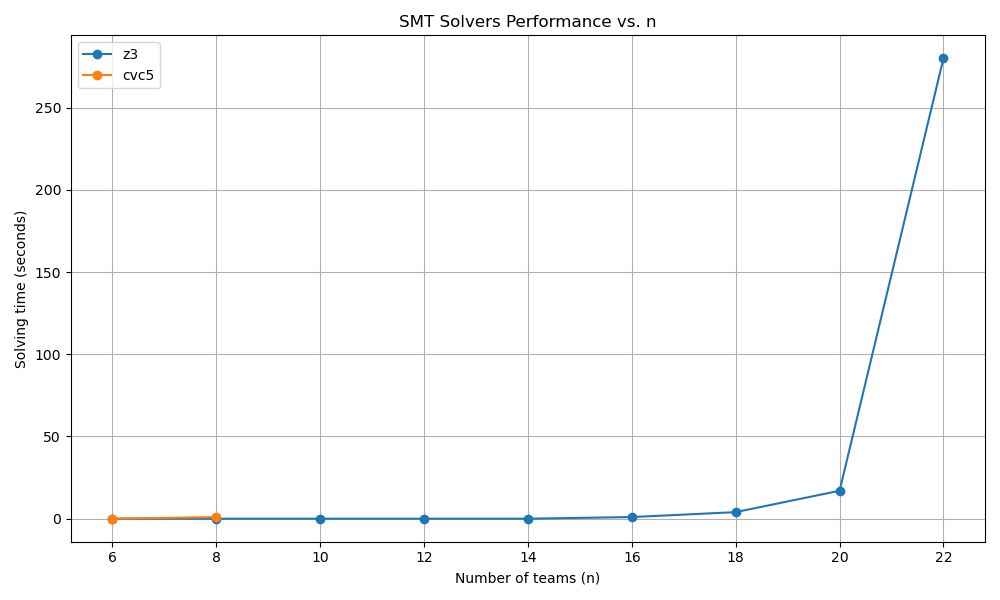
\includegraphics[width=0.8\textwidth]{img/SMT-result.png}
  \caption{SMT Optimization}
  \label{fig:output}
\end{figure}
